\section{实证结果：影响因素}
\label{sec:factors}

本节报告门控组合的基准表现，说明识别策略，并逐个检验四类影响因素：
训练目标、市场环境（含外生冲击）、收益来源渠道与制度持续性。

\begin{table}[htbp]
\centering
\caption{滚动样本外表现（2014--2025 年）}
\label{tab:main}
\begin{threeparttable}
\footnotesize
\begin{tabular}{lrrrr}
\toprule
\multicolumn{5}{l}{\textit{Panel A：收益与风险}} \\
模型 & CAGR & 波动率 & 夏普 & Sortino \\
\midrule
低波动专家 & 0.1285 & 0.1879 & 0.804 & 1.729 \\
风险平价 & 0.1216 & 0.2033 & 0.769 & 1.638 \\
门控组合（主动目标） & 0.1443 & 0.2376 & 0.673 & 2.779 \\
反转专家 & 0.1086 & 0.2691 & 0.579 & 2.055 \\
梯度提升树 & 0.0960 & 0.2369 & 0.566 & 2.148 \\
岭回归 & 0.0955 & 0.2367 & 0.563 & 2.130 \\
等权基准 & 0.0946 & 0.2368 & 0.558 & 2.141 \\
静态专家合成 & 0.1052 & 0.2349 & 0.547 & 1.045 \\
低换手专家 & 0.1018 & 0.2419 & 0.491 & 2.429 \\
动量专家 & 0.1144 & 0.2733 & 0.369 & 0.632 \\
低 beta 专家 & 0.0656 & 0.2410 & 0.351 & 1.528 \\
\bottomrule
\end{tabular}

\vspace{0.5em}
\begin{tabular}{lrrr}
\toprule
\multicolumn{4}{l}{\textit{Panel B：交易摩擦与主动暴露}} \\
模型 & 最大回撤 & 换手率 & 主动暴露 \\
\midrule
低波动专家 & $-0.120$ & 0.257 & 0.488 \\
风险平价 & $-0.133$ & 0.213 & 0.334 \\
门控组合（主动目标） & $-0.155$ & 0.372 & 0.309 \\
反转专家 & $-0.189$ & 0.618 & 0.490 \\
梯度提升树 & $-0.164$ & 0.131 & 0.005 \\
岭回归 & $-0.164$ & 0.131 & 0.005 \\
等权基准 & $-0.164$ & 0.131 & 0.000 \\
静态专家合成 & $-0.164$ & 0.289 & 0.242 \\
低换手专家 & $-0.171$ & 0.297 & 0.315 \\
动量专家 & $-0.197$ & 0.426 & 0.427 \\
低 beta 专家 & $-0.176$ & 0.185 & 0.164 \\
\bottomrule
\end{tabular}
\begin{tablenotes}[flushleft]\footnotesize
\item 注：样本为沪深 A 股点时面板，频率为月度，测试年份 2014--2025 年共 12 个年度窗口，
每个窗口独立重估（训练 5 年、验证 1 年）；学习模型在每个窗口使用三个随机种子并先取平均。
收益指标扣除单边 10 个基点的交易成本。主动暴露为组合权重相对等权的半 $L_1$ 距离均值，
取值范围为 0 至 1，等权组合取 0。2014 年前的年份用于训练与验证，不进入报告。
\end{tablenotes}
\end{threeparttable}
\end{table}

表 \ref{tab:main} 显示，门控组合的主动调整是实质性的：主动暴露为 0.309，
平均约 31\% 的组合权重偏离等权。梯度提升树与岭回归的主动暴露仅为 0.005。
在这两个模型中，直接预测收益再映射为权重的做法产生极端集中的权重，
在不可交易与成本约束下退化为近似等权。若研究者只报告夏普比率而不报告主动暴露，
读者无法区分自适应机制奏效与机制退化。

门控组合取得最高的年化收益（14.43\%）与最高的 Sortino 比率（2.779），
夏普比率 0.673 高于等权基准 0.558 与静态专家合成 0.547。其波动率（0.238）
略高于等权（0.237），收益改善并非来自降杠杆。五个专家信号表现分化明显：
低波动专家（0.804）与风险平价（0.769）优于门控组合，动量专家（0.369）与
低 beta 专家（0.351）明显落后。信号集合的高度异质性正是门控机制的设计场景。

\begin{table}[htbp]
\centering
\caption{相对等权基准的夏普差值检验（配对单位：测试年份，$n=12$）}
\label{tab:signif}
\begin{threeparttable}
\footnotesize
\begin{tabular}{lrrrrc}
\toprule
模型 & 差值 & 95\% 区间下限 & 95\% 区间上限 & 区间含零 & Holm 校正 $p$ \\
\midrule
低波动专家 & $+0.246$ & $+0.123$ & $+0.375$ & 否 & 0.041 \\
风险平价 & $+0.211$ & $+0.130$ & $+0.298$ & 否 & 0.017 \\
门控组合 & $+0.115$ & $-0.006$ & $+0.225$ & 是 & 0.386 \\
反转专家 & $+0.021$ & $-0.109$ & $+0.154$ & 是 & 1.000 \\
梯度提升树 & $+0.008$ & $+0.005$ & $+0.011$ & 否 & 0.005 \\
岭回归 & $+0.005$ & $+0.003$ & $+0.007$ & 否 & 0.009 \\
静态专家合成 & $-0.012$ & $-0.097$ & $+0.064$ & 是 & 1.000 \\
低换手专家 & $-0.067$ & $-0.224$ & $+0.062$ & 是 & 1.000 \\
动量专家 & $-0.190$ & $-0.442$ & $+0.021$ & 是 & 0.934 \\
低 beta 专家 & $-0.207$ & $-0.337$ & $-0.102$ & 否 & 0.009 \\
\bottomrule
\end{tabular}
\begin{tablenotes}[flushleft]\footnotesize
\item 注：区间由循环区块自助法（块长 2 年，10\,000 次重抽样）构造；
$p$ 值为 Wilcoxon 符号秩检验并作 Holm 多重比较校正。Friedman 检验统计量 39.11
（$p<0.001$），模型整体排序存在差异。
\end{tablenotes}
\end{threeparttable}
\end{table}

表 \ref{tab:signif} 报告的夏普差值为 $+0.115$，95\% 区间 $[-0.006,0.225]$，
Wilcoxon $p=0.077$，Holm 校正后 $p=0.386$；对应年化主动收益 3.77\%、
主动信息比率 0.80。门控组合的经济量级明显，统计显著性不足。
低波动专家与风险平价的优势在 5\% 水平上稳健显著（Holm $p=0.041$ 与 $0.017$）。

梯度提升树与岭回归的 Holm $p$ 值分别为 0.005 与 0.009，低于门控组合，
但其绝对量级仅为 $+0.008$ 与 $+0.005$，主动暴露接近零。这两个估计的显著性来自
极小的方差，对应的经济优势有限。仅依赖 $p$ 值判断会得出与量级相反的排序，
本文因此同时报告经济量级与主动暴露。

风险维度提供了另一组信息。门控组合相对等权的日频 5\% CVaR 改善为 $+0.0047$
（95\% 区间 $[-0.0087,0.0181]$），换手率提高 $+0.241$（Holm $p=0.005$）。
门控以显著更高的交易强度换取了幅度有限、与零不可区分的尾部风险改善。
这一取舍是第 \ref{sec:policy} 节讨论风险管理含义的基础。
\begin{figure}[htbp]
\centering
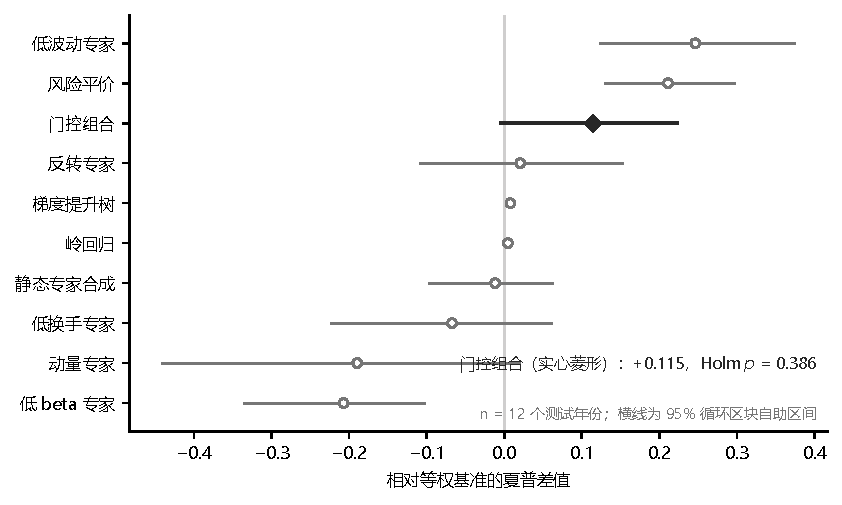
\includegraphics[width=0.82\textwidth]{fig_significance.pdf}
\caption{各模型相对等权基准的夏普差值}
\label{fig:significance}
\begin{minipage}{0.9\textwidth}\footnotesize
注：标记为夏普差值的点估计，横线为循环区块自助法（块长 2 年，10\,000 次重抽样）
构造的 95\% 区间，配对单位为测试年份（$n=12$）；实心菱形为门控组合。
区间跨越零的模型，其优势与零不可区分。
\end{minipage}
\end{figure}

识别策略。门控价值的因果解释面临两个威胁：门控收益可能来自样本内过拟合，
也可能来自与制度无关的风险暴露。本文用三层设计逐一排除。

第一层是随机化推断。按推论 \ref{cor:identification}，
破坏制度与收益的对应关系后门控收益应当归零。本文保持门控输入形式与专家权重不变，
对收益矩阵做循环区块置换并重新训练门控，重复 200 次，得到门控收益的零分布。
该层识别的是制度信息对收益的必要性。

第二层是上界检验。Oracle 门控使用制度内真实条件期望收益，
给出利用一阶互补性所能达到的上界。若门控收益来自收益择时的预测能力，
其表现不应超过该上界。该层识别的是收益来源渠道。

第三层是外生冲击分组。制度切换的时点若由市场内生决定，
「门控在制度切换后表现更好」存在反向因果的可能。
本文改用事件时间外生的冲击年份作为分组变量（政策与国际事件的发生时点不依赖模型），
比较冲击年与对照年的门控价值，并同时检查两组的波动率与切换次数，
以区分状态分化幅度与切换频率两个渠道。

三层设计对应三个识别对象：制度信息的必要性、收益来源渠道、价值的时点分布。
任何单层都不足以构成因果论证，合起来可以排除过拟合、渠道误判与内生时点三个主要解释。
识别仍依赖的前提是：专家信号的方向由理论事先设定、不参与自由训练；
门控只在训练窗内拟合，验证窗选超参，测试窗仅用于评估。

\begin{table}[htbp]
\centering
\caption{训练目标对门控行为的影响}
\label{tab:degeneracy}
\begin{threeparttable}
\footnotesize
\begin{tabular}{p{2.9cm}rrrp{2.4cm}}
\toprule
训练目标 & 主动暴露 & 平均换手率 & 相对等权的夏普差 & 结论 \\
\midrule
绝对收益（常见做法） & $\approx0.0003$ & 0.0029 & $-0.001$（含零，$p=1.000$） & 退化为静态等权 \\
主动收益（本文修正） & 0.309 & 0.372 & $+0.115$（含零，$p=0.077$） & 实质动态调整 \\
\bottomrule
\end{tabular}
\begin{tablenotes}[flushleft]\footnotesize
\item 注：绝对收益目标的行为来自以十只美国 ETF 为样本的设定；
主动收益目标的行为来自本文的 A 股主实验。主动暴露为组合权重相对等权的半 $L_1$ 距离。
\end{tablenotes}
\end{threeparttable}
\end{table}

表 \ref{tab:degeneracy} 对比两种训练目标下的门控行为，用于检验命题 \ref{prop:degeneracy}。
绝对收益目标下，主动暴露约为 $0.0003$，组合几乎恒等于等权；换手率 0.0029
与静态持有水平相当；夏普比率与等权基准无法区分。目标函数中与决策无关的基准收益项
主导梯度，是该行为的直接来源。改为主动收益目标后，主动暴露上升约三个数量级至 0.309，
门控具备识别互补性的条件。

这一对照的适用范围超出本文样本。在满仓长仓约束下，训练目标的选择决定自适应机制
能否偏离静态基准，其影响先于网络架构的设计。使用绝对收益目标的同类研究，
若不报告主动暴露，其零结果可能来自目标函数设计而非机制无效。报告自适应组合表现时
同时报告主动暴露，可以把这一来源区分开。

\begin{table}[htbp]
\centering
\caption{年度市场环境与门控组合的相对表现}
\label{tab:year-env}
\begin{threeparttable}
\footnotesize
\begin{tabular}{lrrrrrrr}
\toprule
年份 & 市场收益 & 市场波动率 & 制度切换次数 & 横截面离散度
& 门控夏普 & 等权夏普 & 夏普差值 \\
\midrule
2014 & 0.427 & 0.148 & 1 & 0.105 & 2.587 & 2.491 & $+0.096$ \\
2015 & 0.040 & 0.575 & 1 & 0.137 & 0.515 & 0.367 & $+0.148$ \\
2016 & 0.224 & 0.177 & 5 & 0.090 & 1.410 & 1.221 & $+0.189$ \\
2017 & $-0.135$ & 0.188 & 4 & 0.091 & $-0.497$ & $-0.682$ & $+0.185$ \\
2018 & $-0.271$ & 0.176 & 0 & 0.091 & $-1.445$ & $-1.691$ & $+0.246$ \\
2019 & 0.127 & 0.328 & 3 & 0.102 & 0.722 & 0.509 & $+0.214$ \\
2020 & 0.187 & 0.285 & 7 & 0.124 & 1.030 & 0.725 & $+0.305$ \\
2021 & 0.203 & 0.165 & 6 & 0.130 & 1.554 & 1.199 & $+0.355$ \\
2022 & 0.034 & 0.241 & 3 & 0.120 & 0.186 & 0.210 & $-0.024$ \\
2023 & $-0.233$ & 0.164 & 3 & 0.088 & $-1.790$ & $-1.523$ & $-0.267$ \\
2024 & 0.208 & 0.324 & 2 & 0.115 & 0.786 & 0.698 & $+0.088$ \\
2025 & 0.347 & 0.096 & 4 & 0.112 & 3.013 & 3.174 & $-0.162$ \\
\bottomrule
\end{tabular}
\begin{tablenotes}[flushleft]\footnotesize
\item 注：市场收益为上证与深证综合口径的年度累计收益，市场波动率为月度收益标准差年化，
制度切换次数为 12 个月市场收益三分位制度在年内发生变化的次数，
横截面离散度为个股月收益横截面标准差的时间均值。门控夏普为三个随机种子的年内均值。
\end{tablenotes}
\end{threeparttable}
\end{table}

表 \ref{tab:year-env} 与图 \ref{fig:determinants} 报告门控相对价值的年度分布。
门控的相对价值随市场分化程度上升。年度波动率最低的三分之一年份，
夏普差值平均为 $+0.006$；中间三分之一为 $+0.149$；最高的三分之一为 $+0.189$，
秩相关系数为 0.259。横截面离散度呈现同向特征：最低三分之一为 $+0.088$，
最高三分之一为 $+0.196$，秩相关为 0.231。市场方向不解释门控价值：
年度收益与差值的秩相关为 $-0.049$，年度最大回撤为 0.042。
门控价值来自市场状态的分化程度，而非市场涨跌。

\begin{figure}[htbp]
\centering
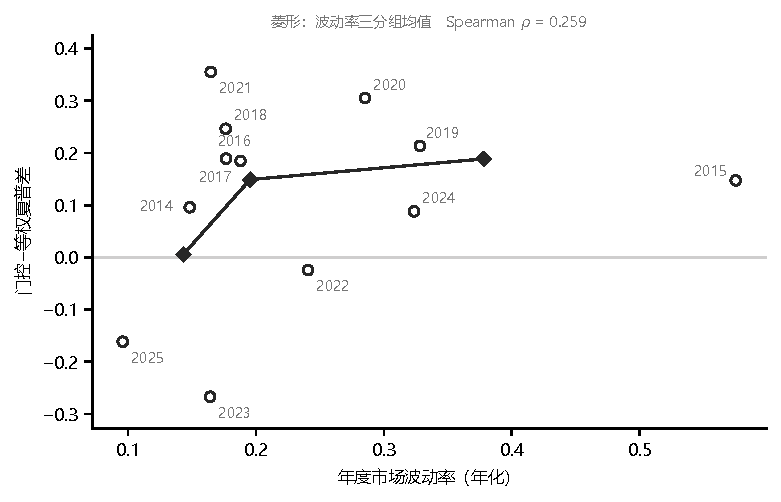
\includegraphics[width=0.78\textwidth]{fig_determinants.pdf}
\caption{年度市场波动率与门控组合的相对优势（2014--2025 年）}
\label{fig:determinants}
\begin{minipage}{0.86\textwidth}\footnotesize
注：散点为 12 个测试年份，纵轴为门控组合相对等权基准的夏普差值；
折线为按年度波动率三分组的组内均值。$N=12$。
\end{minipage}
\end{figure}

年度观测只有 12 个，单变量回归不足以支持因果推断，上述分组特征作为门控优势
在时间上分布不均衡的证据，其方向与「制度条件信息在高波动、高分化环境下更有价值」
的机制一致。

外生冲击下的门控价值。表 \ref{tab:year-env} 的分组变量由市场统计量构造，可能与门控表现同时受第三方因素影响。
本节改用事件时间外生的冲击年份作分组，冲击的发生时点由政策与国际事件决定，
不依赖模型与策略。

\begin{table}[htbp]
\centering
\caption{外生冲击年与对照年的门控价值}
\label{tab:shock}
\begin{threeparttable}
\small
\begin{tabular}{lrrrr}
\toprule
分组 & 夏普差值均值 & 市场波动率 & 制度切换次数 & 横截面离散度 \\
\midrule
冲击年（5 个） & $+0.173$ & 0.291 & 3.20 & 0.112 \\
对照年（7 个） & $+0.073$ & 0.202 & 3.29 & 0.106 \\
\midrule
\multicolumn{5}{l}{差值（年份聚类自助，2\,000 次）：
$+0.100$，95\% 区间 $[-0.081,0.276]$，$p=0.298$} \\
\bottomrule
\end{tabular}
\begin{tablenotes}[flushleft]\footnotesize
\item 注：冲击年为 2015、2016、2018、2020、2022 年，依次对应股市异常波动、
熔断机制实施、中美贸易摩擦、新冠疫情、俄乌冲突与疫情封控，
事件时点由外部事件日历确定；其余 7 年为对照年。
市场波动率为月度收益标准差年化，制度切换次数为 12 个月市场收益三分位制度
在年内发生变化的次数，横截面离散度为个股月收益横截面标准差的时间均值。
夏普差值为门控组合相对等权基准的差值。
\end{tablenotes}
\end{threeparttable}
\end{table}

冲击年的门控相对优势为 $+0.173$，对照年为 $+0.073$，差值为 $+0.100$
（95\% 区间 $[-0.081,0.276]$）。点估计方向与「外生冲击提高状态分化程度、
从而提高门控价值」的推断一致，区间的宽度说明 12 个年度观测下的识别能力有限。
两组的分组特征给出机制信息：冲击年的市场波动率为 0.291，明显高于对照年的 0.202；
制度切换次数几乎相同（3.20 对 3.29）；横截面离散度略高（0.112 对 0.106）。
门控价值与状态分化的幅度同向，与制度切换的频率关系不大，
这与前文的结果一致。该模式同时排除一类解释：
门控收益并非来自频繁调仓本身。

门控的可实施性还取决于状态能否实时识别。若状态切换可以被事前预判，
策略可以通过择时调仓规避高成本时段；若不能，门控的价值只能来自识别当前状态并利用其持续性。
本文用 logit 与 probit 模型检验这一问题，被解释变量为下月状态，
解释变量为滞后一期的公开信息，结果见表 \ref{tab:logit}。

三个结果值得注意。制度切换基本不可预测：伪 $R^2$ 为 0.04，
样本内命中率 0.53 低于「始终预测不切换」的 0.76，切换时点没有可用的公开前兆。
状态本身具有很强的判别力：风险结构制度的伪 $R^2$ 为 0.45、样本外命中率 0.87，
收益水平制度为 0.41、0.75。判别力的来源符合渠道分解：
风险结构制度的主要判别变量是滞后波动率（平均边际效应 $+0.194$，$p<0.001$），
即波动聚集；收益水平制度的主要判别变量是滞后回撤（$-0.314$，$p<0.001$）
与横截面离散度（$-0.138$，$p<0.001$），其余变量的边际效应在 10\% 水平上不显著。

这组结果与持续性乘数一致：状态的价值来自其持续性，而非对切换时点的预知。
门控因此是可实施的——策略不需要预测何时切换，只需在每月识别当前状态；
但它也无法通过择时规避切换带来的换手成本，这与第 \ref{sec:marginal} 节的
成本敏感性结果互相呼应。

\begin{table}[htbp]
\centering
\caption{状态可预测性检验（被解释变量：下月状态）}
\label{tab:logit}
\begin{threeparttable}
\footnotesize
\begin{tabular}{lrrrr}
\toprule
被解释变量 & 模型 & 伪 $R^2$ & 样本内命中率 & 样本外命中率 \\
\midrule
风险结构制度（高波动） & logit & 0.449 & 0.834 & 0.874 \\
风险结构制度（高波动） & probit & 0.436 & 0.834 & 0.869 \\
收益水平制度（熊市） & logit & 0.406 & 0.809 & 0.754 \\
收益水平制度（熊市） & probit & 0.413 & 0.809 & 0.760 \\
制度切换（收益水平划分） & logit & 0.041 & 0.528 & 0.726 \\
制度切换（收益水平划分） & probit & 0.042 & 0.532 & 0.726 \\
\midrule
\multicolumn{5}{l}{基准率：风险结构制度 0.32、收益水平制度 0.34、制度切换 0.24} \\
\bottomrule
\end{tabular}
\begin{tablenotes}[flushleft]\footnotesize
\item 注：样本为 2006--2026 年 235 个月度观测；解释变量为滞后一期的公开信息
（上月市场收益、近 3 个月收益、近 6 个月波动、近 1 年回撤、横截面离散度、
上涨股票占比），均做标准化处理；标准误为 Newey--West（6 阶）。
样本外命中率为扩展窗逐步预测的结果，训练起点为第 60 个月。
基准率指被解释变量取 1 的无条件频率。
\end{tablenotes}
\end{threeparttable}
\end{table}

\begin{table}[htbp]
\centering
\caption{信号—状态互补性与估计噪声底线}
\label{tab:gamma}
\begin{threeparttable}
\small
\begin{tabular}{llrrrr}
\toprule
估计口径 & 渠道 & 统计量 & 噪声底线 $\Theta$ & $p$ 值 & 是否越过 5\% \\
\midrule
截面回归 IC & 一阶 & $4.0\times10^{-6}$ & $1.4\times10^{-5}$ & 0.708 & 否 \\
专家组合收益 & 一阶 & $3.93\times10^{-4}$ & $4.17\times10^{-4}$ & 0.060 & 否（临界） \\
专家组合收益 & 二阶 & $6.34\times10^{-4}$ & $6.87\times10^{-4}$ & 0.065 & 否（临界） \\
\midrule
\multicolumn{2}{l}{美国 ETF 10 只（$N=10$）} & \multicolumn{3}{r}{不可识别} & —— \\
\bottomrule
\end{tabular}
\begin{tablenotes}[flushleft]\footnotesize
\item 注：$\Theta$ 由循环区块自助法在「无真实互补性」原假设下校准
（块长 6--12 个月，500 次重抽样），取统计量分布的 95\% 分位数；
$p$ 值为自助分布中不小于观测值的比例。窄横截面样本因每月证券数不足 20 只
而无法估计月度横截面回归。
\end{tablenotes}
\end{threeparttable}
\end{table}

表 \ref{tab:gamma} 的三种口径给出一致结果：互补性统计量均未越过 5\% 水平的噪声底线，
两种专家组合收益口径接近临界（一阶 $p=0.060$，二阶 $p=0.065$）。
在 12 个测试年份、247 个月度观测下，条件信息系数的制度间差异刚好处在
可与抽样噪声区分的边缘。该结果与表 \ref{tab:signif} 中 $+0.115$ 的夏普差值互相印证，
两套独立检验给出同一个位置判断：门控运行在阈值附近。

\begin{table}[htbp]
\centering
\caption{渠道识别：Oracle 上界、安慰剂与变异系数检验}
\label{tab:oracle}
\begin{threeparttable}
\small
\begin{tabular}{lrrr}
\toprule
检验 & 夏普 & 年化收益 & 换手率 \\
\midrule
等权基准 & 0.558 & 9.5\% & 0.131 \\
静态专家合成 & 0.546 & 10.5\% & 0.289 \\
Oracle 门控（用真实条件期望收益） & 0.562 & 10.7\% & 0.291 \\
\midrule
\multicolumn{4}{l}{\textit{安慰剂检验（区块置换收益—制度关联，200 次）}} \\
门控主动收益 & \multicolumn{3}{r}{$+0.004\%$，95\% 区间 $[-0.413\%,+0.357\%]$} \\
\midrule
\multicolumn{4}{l}{\textit{渠道识别检验（区块置换，1\,000 次，块长 12 月）}} \\
一阶变异系数 $\mathrm{CV}^{(1)}$ & \multicolumn{3}{r}{观测 2.722 vs 零分布均值 0.450，$p=0.001$} \\
二阶变异系数 $\mathrm{CV}^{(2)}$ & \multicolumn{3}{r}{观测 0.104 vs 零分布均值 0.022，$p=0.003$} \\
\bottomrule
\end{tabular}
\begin{tablenotes}[flushleft]\footnotesize
\item 注：Oracle 门控按训练窗内各制度的资产平均持有期收益为专家加权，
使用真实条件期望收益，不可实现，仅用于构造一阶互补性的可利用上界。
变异系数定义为制度间方差除以均值平方。
\end{tablenotes}
\end{threeparttable}
\end{table}

表 \ref{tab:oracle} 的三类检验依次确定收益的制度依赖、来源渠道与状态依赖强度。
安慰剂检验把门控主动收益由 3.77\% 压至 0.004\%（95\% 区间 $[-0.413\%,+0.357\%]$），
按推论 \ref{cor:identification}，门控收益依赖制度信息，不是样本内过拟合或随机噪声。
Oracle 门控的夏普比率为 0.562，与等权基准（0.558）和静态专家合成（0.546）几乎无差异：
即使允许门控使用各制度内真实的条件期望收益，表现也没有改善，
数据中可利用的一阶互补性有限。渠道识别检验显示制度间变异系数远超置换零分布，
一阶 $\mathrm{CV}^{(1)}$ 为 2.722（零分布均值 0.450，$p=0.001$），
二阶 $\mathrm{CV}^{(2)}$ 为 0.104（零分布均值 0.022，$p=0.003$），
两条渠道都存在显著的状态依赖。

三类检验合起来指向同一结论：状态依赖存在，可利用的一阶互补性有限，
门控收益主要来自二阶渠道，即通过识别制度相关的风险结构
（专家信号的波动率与相关性差异）重新配置风险，而非预测哪个专家在哪个制度下收益更高。
该结论有一个直接推论：若门控价值主要来自风险配置，更简单的风险结构策略应当同样有效。
表 \ref{tab:main} 与此一致：低波动专家（0.804）与风险平价（0.769）都是二阶渠道的
纯化形式，表现优于包含完整门控机制的组合（0.673）。

\begin{figure}[htbp]
\centering
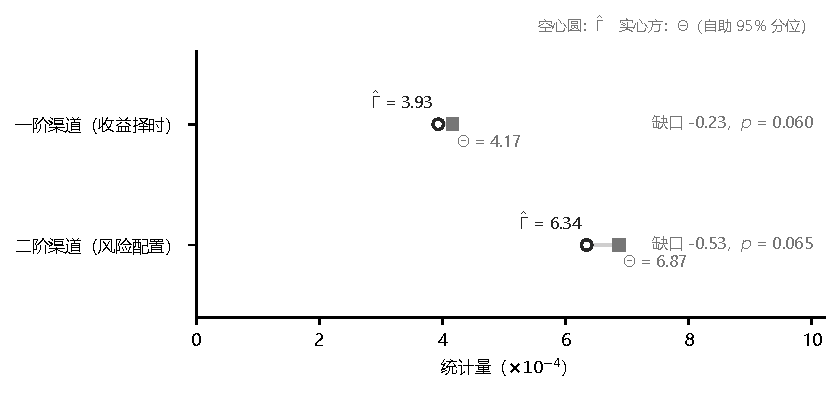
\includegraphics[width=0.62\textwidth]{fig_threshold.pdf}
\caption{互补性统计量与噪声底线的对照}
\label{fig:threshold}
\begin{minipage}{0.86\textwidth}\footnotesize
注：白色阴影柱为互补性统计量 $\hat\Gamma$，灰色柱为循环区块自助法校准的
噪声底线 $\Theta$（95\% 分位）。两条渠道的 $\hat\Gamma$ 均略低于 $\Theta$。
\end{minipage}
\end{figure}

\begin{table}[htbp]
\centering
\caption{制度转移矩阵与持续性乘数（三制度，按 12 个月市场收益分位划分）}
\label{tab:persistence}
\begin{threeparttable}
\small
\begin{tabular}{lrrrrr}
\toprule
& \multicolumn{3}{c}{转移概率} & 持续概率 & 半衰期（月） \\
\cmidrule(lr){2-4}
制度 & 下一期=1 & 下一期=2 & 下一期=3 & & \\
\midrule
1（熊市） & 0.829 & 0.171 & 0.000 & 0.829 & 3.70 \\
2（震荡） & 0.148 & 0.704 & 0.148 & 0.704 & 1.97 \\
3（牛市） & 0.024 & 0.133 & 0.843 & 0.843 & 4.07 \\
\midrule
\multicolumn{5}{l}{平稳分布} & (0.340, 0.339, 0.321) \\
\multicolumn{5}{l}{持续性乘数 $\mathcal{M}_s$（$\beta=0.98$）} & (19.81, 18.40, 19.16) \\
\multicolumn{5}{l}{$\Corr(\mathcal{M}_s,\ \Gamma^{(1)}_s)$} & 0.985 \\
\multicolumn{5}{l}{持续性加权 / 未加权 $\Gamma^{(1)}$} & $19.5\times$ \\
\bottomrule
\end{tabular}
\begin{tablenotes}[flushleft]\footnotesize
\item 注：半衰期 $h_s=\ln0.5/\ln p_{ss}$；
持续性乘数 $\mathcal{M}_s=[(I-\beta P)^{-1}]_{ss}$，度量掌握当前制度对未来
收益分布的信息价值。
\end{tablenotes}
\end{threeparttable}
\end{table}

中国 A 股的制度状态高度持续：表 \ref{tab:persistence} 中转移矩阵的对角线概率为
0.829、0.704、0.843，平均半衰期 3.25 个月。「当前制度」包含关于未来 1--4 个月
收益分布的实质信息，而非瞬时噪声。持续性乘数与制度条件互补性的相关系数为 0.985，
考虑持续性后加权互补性为未加权的 19.5 倍，与定理 \ref{thm:persistence} 的方向一致。
持续性放大的是门控价值的量级，不改变阈值判定，因为噪声底线同样受制度内样本量约束。
$S=3$ 时上述相关系数只有 3 个观测点，此处作为方向性证据，不作精确估计。

识别设计给出三点支持：安慰剂检验排除样本内过拟合，Oracle 上界排除收益择时主导，
外生冲击分组把价值的时点分布与状态分化幅度而非切换频率联系起来。
在此基础上，四类影响因素按作用次序排列：训练目标决定机制能否偏离静态基准，
是必要条件；市场分化程度决定相对价值的年度分布；收益来源渠道决定门控的可实现形式
是风险结构配置；制度持续性放大价值量级。前三类因素都指向同一判断：
门控的价值来自信号的制度差异，而非信号数量或模型复杂度。
